\chapter{Adversarial Tracking}
\label{chpt:tracking}

% \newrefsection

In this chapter, we present adversarial attacks against object tracking systems. Unlike object detection systems that only make predictions based on the current input image from the camera, object tracking models combine prior predictions with current inputs to generate trajectories of moving objects, making it more challenging to achieve adversarial attacks.

\section{Adversarial Tracking}
\label{sec:adv_track}

As introduced in the first chapter, deep learning models have been widely adopted in autonomous driving for perception tasks. For example, object tracking models are utilized to generate trajectories of moving objects. Under this scenario, we do not have access to gradients, making white-box attacks virtually impossible, neither do we have access to query results that are intermediate results in the internal data path.

\begin{figure}[b]
\centering
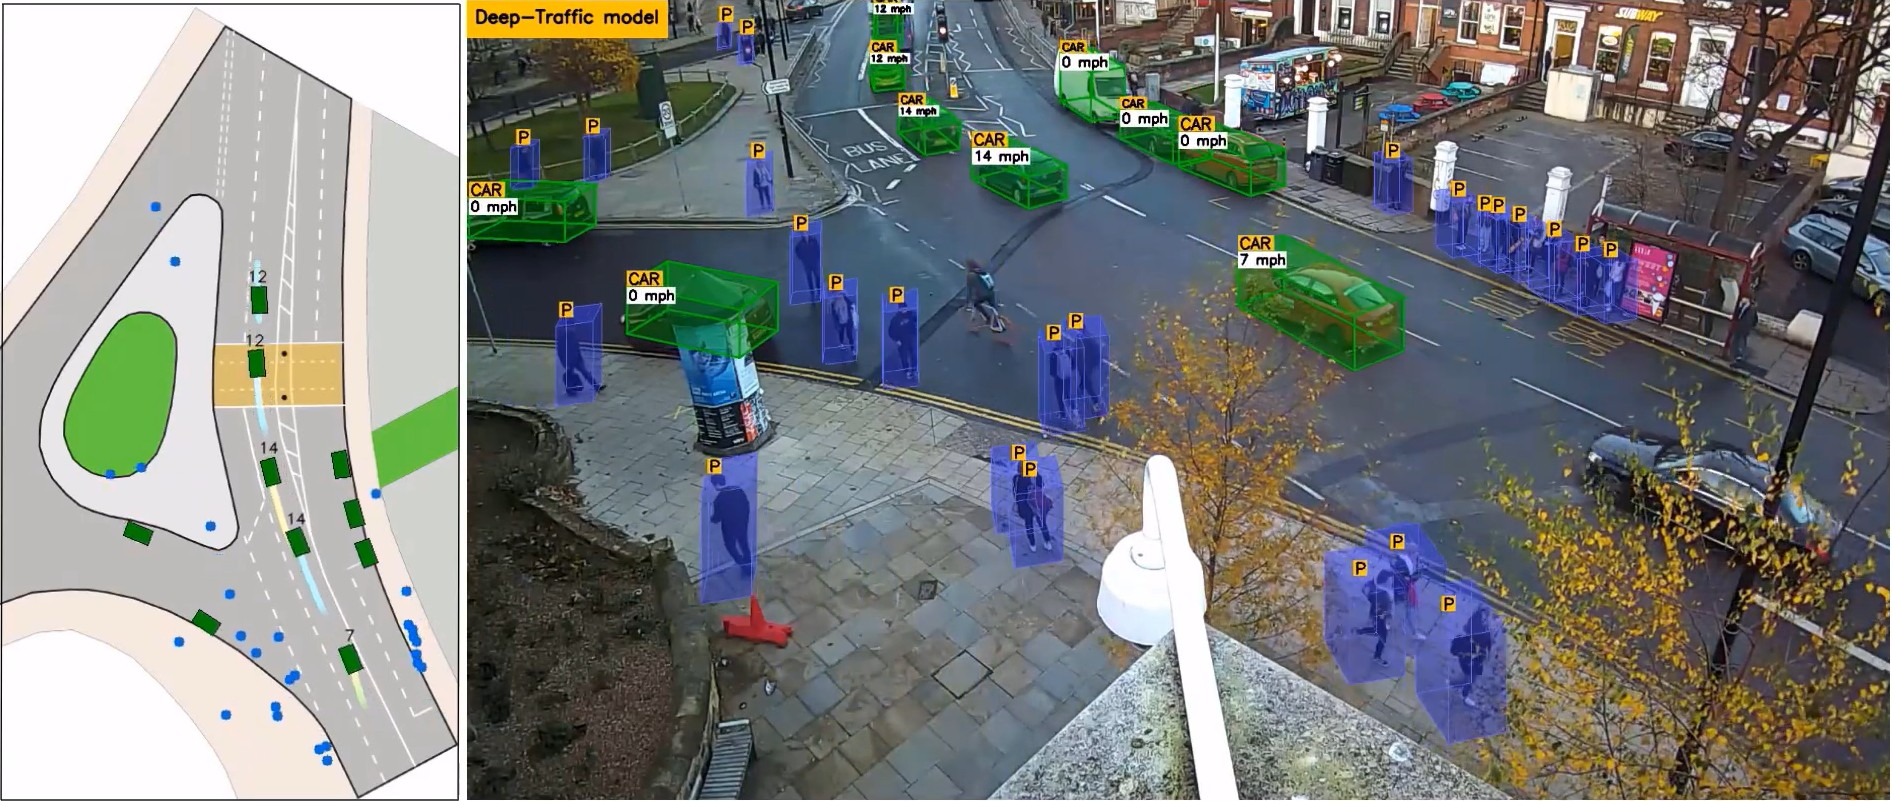
\includegraphics[width=0.7\textwidth]{figures/chapter_4/tracking.jpg}
\caption{2D Object Detection and Tracking using YOLO4 in Autonomous Vehicles}
\label{fig.tracking}
\end{figure}

% \begin{figure}[H]
% \centering
% \begin{subfigure}[b]{0.485\textwidth}
%     \centering
%     \includegraphics[width=\textwidth]{chapters/figures/frame_0.jpg}
%     \caption{Sequence 0, Frame 1 }
%     \label{fig:frame_0}
% \end{subfigure}
% \hfill
% \begin{subfigure}[b]{0.485\textwidth}
%     \centering
%     \includegraphics[width=\textwidth]{chapters/figures/frame_1.jpg}
%     \caption{Sequence 0, Frame 2}
%     \label{fig:frame_1}
% \end{subfigure}
% \hfill
% \caption{Realtime Object Tracking \citep{chiu2020probabilistic}}
% \label{fig.obj_track}
% \end{figure}

\begin{table}[H]
\centering
\begin{tabular}{ ccc } 
\hline
Rank & Model & Popularity \\
\hline
1 & SSD & 605 \\ 
2 & YOLO-v3 & 251 \\ 
3 & Faster R-CNN & 236 \\ 
4 & R-CNN & 178 \\ 
5 & YOLO-v2 & 164 \\ 
6 & RetinaNet & 75 \\ 
7 & Yolo-v1 & 52 \\ 
\hline
\end{tabular}
\caption{Object detection models on Github  \citep{wang2021daedalus}}
\label{tab.detection_github}
\end{table}

Does this mean current autonomous driving systems are robust against adversarial attacks? Possibly not. Because object tracking systems still use similar pre-trained object detection models (see Tab.\ref{tab.detection_github}), which means the perturbation generated from object detection models can possibly be applied to object tracking systems.

In the next step, we plan to implement a real-time object tracking system. Then we can investigate the effect of hardware acceleration on the robustness of the model, and if it's possible to attack such a system without prior knowledge of the structure of the model.

%%%%%%%%% BODY TEXT
\section{Preliminaries}
\label{sec:intro}

The first tracking system used radar and sonar to track objects for military applications, and the algorithm consists of four parts: data association, state update, state prediction, and track management. Later, the employment of deep learning yields significant performance increases during data association for visual tracking.

Before the wide adoption of deep learning, it is popular to solve the visual tracking problem using low-level features and statistical learning techniques. Vo et al. reviewed three major techniques used to find the correspondence between detections and tracklet \citep{vo2015multitarget}: The Joint Probabilistic Data Association Filter (JPDAF), Multi Hypothesis Tracking (MHT), and Random Finite Sets (RFS). They also introduced four nonlinear filters: Bayesian Estimation, Kalman Filter, Particle Filter, and the Gaussian Sum Filter.

As research in deep learning advances, Krebs et al. reviewed the application of deep neural networks for object tracking: feature extraction, data association, and end-to-end tracking \citep{krebs2017survey}. Most recent research focuses on tracking pedestrians, and Tracking-By-Detection (TBD) has become the most popular Multi-Object Tracking (MOT) framework. In \citep{sun2020survey}, Sun et al. thoroughly analyzed the current developments in TBD-based MOT algorithms that includes four major components: localization, feature extraction, data association, and tack management.

There is also a growing trend of employing Joint Detection and Tracking (JDT), which is also described as end-to-end tracking in some literature \citep{pal2021deep}. More recently, a review on deep-learning-based visual multi-object tracking algorithms also includes Transformer-based methods \citep{guo2022review}.

% Image Classification: Classify the most salient object of the entire image.

% Object Detection: Classify and Detection the position of each object. (more challenging than classification). We detect the object independently in each frame.

% Object Tracking: Classify and Detect the position of each object as well as estimating the motion model of each object (more challenging than detection).

% Hungarian method was used to find the optimal association to an assignment problem in 2008.

\subsection{Object Tracking}

Recent research interests are shifting from Single Object Tracking (SOT) to Multi-Object Tracking (MOT). For MOT, there are three most popular frameworks:

\begin{itemize}
    \item Tracking by Detection (TBD): A modular framework that heavily relies on the accuracy of the detector, such as SiamRPN++ \citep{li2019siamrpn++} for SOT.
    \item Joint Detection and Tracking (JDT): The end-to-end tracking model is more efficient.
    \item Transformer: More accurate, but computationally expensive \citep{meinhardt2022trackformer} for 2D MOT \citep{lin2021swintrack}.
\end{itemize}

For autonomous driving, it is important to estimate vehicles' pose via 3D Object Tracking, and we plan to focus on vision-only multi-object trackers: 

\begin{itemize}
    \item Multi-Modality Tracker: Associate detection results with 3D Lidar data \citep{weng20203d}.
    \item Monocular Tracker:  Vision-only methods \citep{wu2021track} \citep{hu2022monocular}.
\end{itemize}

In \citep{ciaparrone2020deep}, Ciaparrone et al. listed the most popular evaluation dataset (MOTChallenge, KITTI, nuScenes) and evaluation metrics (MOTA, MOTP, MT, ML, FP, FN).

% Object Tracking Assumptions: 

% \begin{enumerate}
%     \item Camera is not moving instantly to new viewpoint.
%     \item Objects do not disappear and reappear in different places in the scene.
%     \item If the camera is moving, there is a gradual change in pose between camera and scene.
% \end{enumerate}

\subsection{Adversarial Attacks}

The first adversarial attack against MOT attacks a TBD method that uses YOLOv3 as the object detection model, the Hungarian matching for the data association, and the Kalman filter for noisy measurement.

Most following work attacks SiameseRPN-based trackers for SOT \citep{wu2019sta} \citep{liang2020efficient} \citep{guo2020spark} \citep{chen2020one} \citep{yan2020cooling}. Another research attacks the GOTURN model, which is an efficient end-to-end SOT model \citep{wiyatno2019physical}. We only find one research paper that attacks FairMOT (JDT) \citep{lin2021trasw}. There are many adversarial attacks against 3D Lidar Point Cloud \citep{cheng2021universal} \citep{cheng2022non} \citep{wang2022adversary}.

\section{Summary}

In summary, we find several research papers that attack 2D SOT (caemera) and 3D MOT ( Lidar). But we do not find attacks against 3D monocular trackers \citep{wu2021track} \citep{hu2022monocular}. Neither do we find research that attacks Transformers for 2D MOT.

We plan to attack 3D MOT models for Vision-Based vehicle tracking in real time (no 3D Lidar Data). First, we'll implement two 3D MOT models: \href{https://github.com/SysCV/qd-3dt}{QD-3DT} and \href{https://github.com/JialianW/TraDeS}{TraDeS}. Then, we'll try to design white-box attacks to fabricate, vanish 3D bounding boxes, change their orientations, or dissociate them with actual objects.


% \section{Hardware Acceleration}
% \label{sec:hardware}

% % As deep neural networks grow larger to achieve high accuracy on complex tasks, high-performance inference becomes infeasible for traditional general-purpose CPUs. As a result, several neural network hardware accelerator platforms arise, such as graphics processing units (GPUs), field-programmable gate arrays (FPGAs), and application-specific integrated circuits (ASICs). On the other hand, edge devices with limited memory and power supply require a reduced size of models at the cost of acceptable accuracy drop. However, the security and robustness of deep learning applications can be as crucial as accuracy and performance. In our research, we investigate the impact of hardware acceleration on model robustness.

% Traditional general-purpose CPUs use combinations of low-level instructions (x86, x64, MIPS, RISC-V) to implement high-level algorithms. The abstraction from low-level instruction set architecture (ISA) provides compatibility for high-level applications among different hardware. However, there is a trade-off between efficiency and generalization. Software implementation of algorithms is compatible among different hardware, while hardware implementation of algorithms is much more efficient. In the hardware domain, hardware description languages such as VHDL and Verilog are utilized in synthesis and simulation. In the software domain, high-level languages such as C/C++ are commonly used in embedded systems. Requirements for high-speed data exchange, especially for cellular base stations, obscures the boundary between software and hardware.

% During the 1990s, research interest on hardware-software codesign including estimation, exploration, partitioning, interfacing, communication, synthesis, and cosimulation gained momentum \citep{coussy2009introduction}. Around the same time, the first generation of commercial high-level synthesis (HLS) tools was available commercially. High-level synthesis generates optimized RTL hardware using high-level languages. The architecture of generated RTL usually includes a controller and a data path as illustrated in Figure \ref{fig.hls}.


% \begin{figure}[H]
% \centering
% 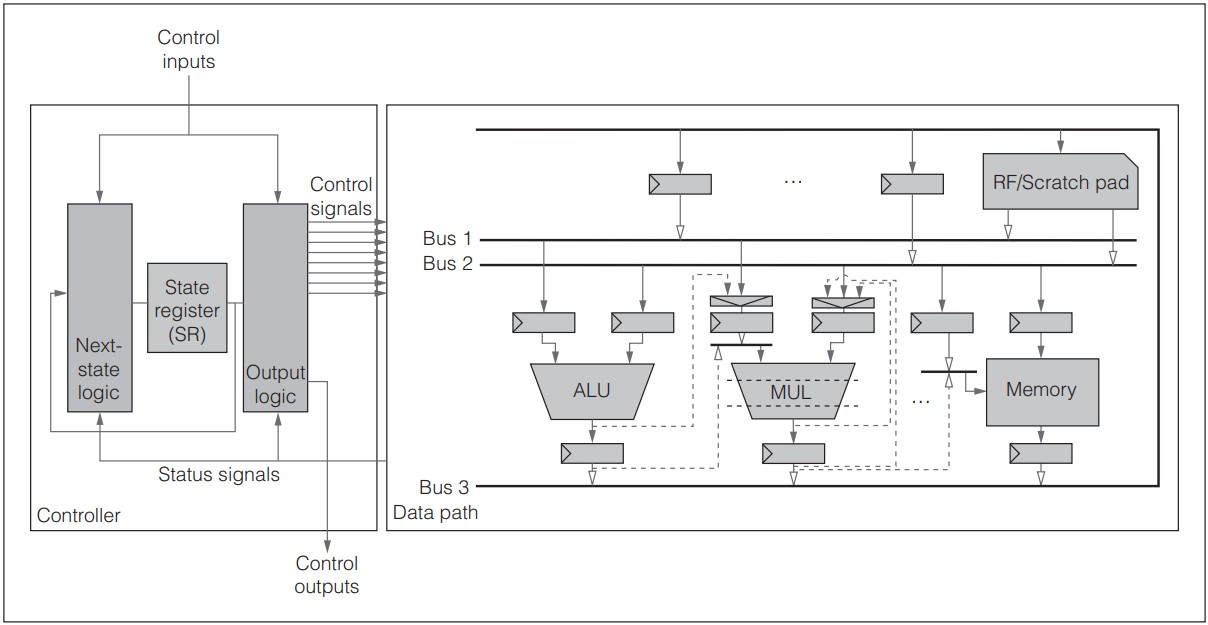
\includegraphics[width=\textwidth]{figures/chapter_4/hls.jpg}
% \caption{Typical Architecture of HLS generated RTL\citep{coussy2009introduction}}
% \label{fig.hls}
% \end{figure}

% \begin{figure}[H]
% \centering
% 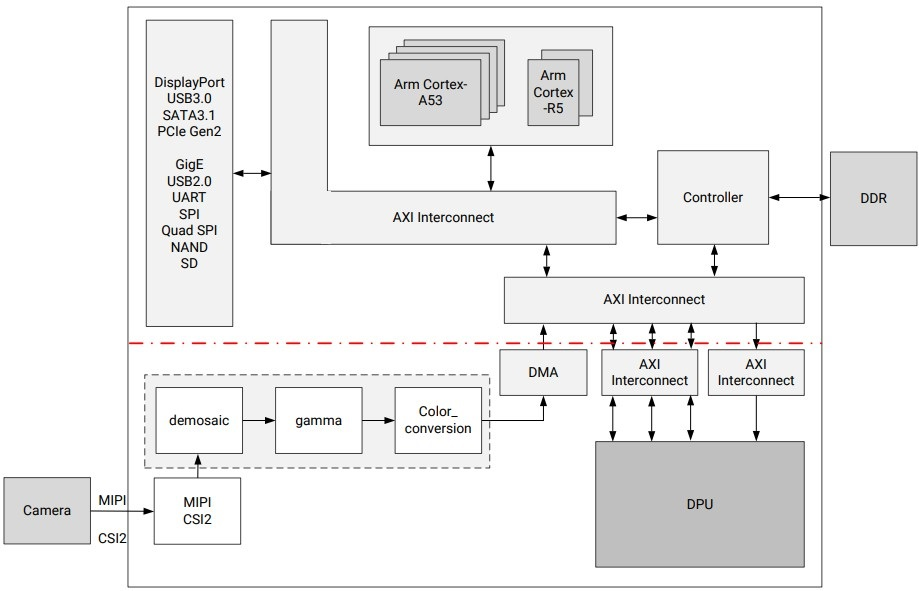
\includegraphics[width=\textwidth]{figures/chapter_4/dpu.jpg}
% \caption{Example System with Integrated DPU \citep{zynq2020}}
% \label{fig.dpu}
% \end{figure}

% As the concept of IP core and platform-based design starts to emerge, now we have dedicated processing units for neural networks. Figure \ref{fig.dpu} illustrates the deployment of deep learning models with hardware acceleration using the Xilinx® Deep Learning Processing Unit (DPU). The DPU implements commonly used operations such as convolution and deconvolution using hardware description language such as Verilog. Then the DPU is released as an intellectual property (IP) and is accessible from the Advanced eXtensible Interface (AXI) bus. Compared with general-purpose CPUs that use combinations of general-purpose instructions to implement convolution, the DPU uses fewer instructions and consumes less energy. The functionality of encapsulated IP Core is accessible from Python libraries using PYNQ, bringing low-level ASIC-style IP cores directly to high-level algorithms.

% \begin{figure}[H]
% \centering
% 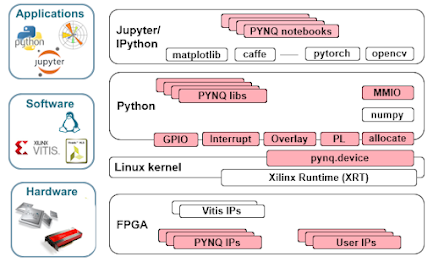
\includegraphics[scale=0.75]{figures/chapter_4/pynq.png}
% \caption{PYNQ: access hardware libraries and overlays for FPGA}
% \label{fig.pynq}
% \end{figure}

% Besides hardware accelerator, edge devices that receive power supply from batteries require deep learning models to be energy-efficient. Quantization and pruning are the two most widely adopted methods to reduce the size of the original model before deploying on real hardware. On the other hand, rather than compress the original model, knowledge distillation effectively learns a small student model from
% a large teacher model to achieve compression and acceleration.

% Quantization uses lower bit integers rather than 32-bit floating points to represent weights and activations. It has been extensively demonstrated that weights and activations can be represented using 8-bit integers (or INT8) without incurring significant loss in accuracy. The use of even lower bit-widths, such as 4/2/1-bits, is an active field of research that has also shown great progress \citep{zmora2019neural}. Quantization reduces energy consumption as well. As illustrated in Figure \ref{fig.quantization}, 32-bit floating point multiplication and memory read consumes 100x-10000x energy than 8-bit operations, as well as more area cost. 

% \begin{figure}[H]
% \centering
% 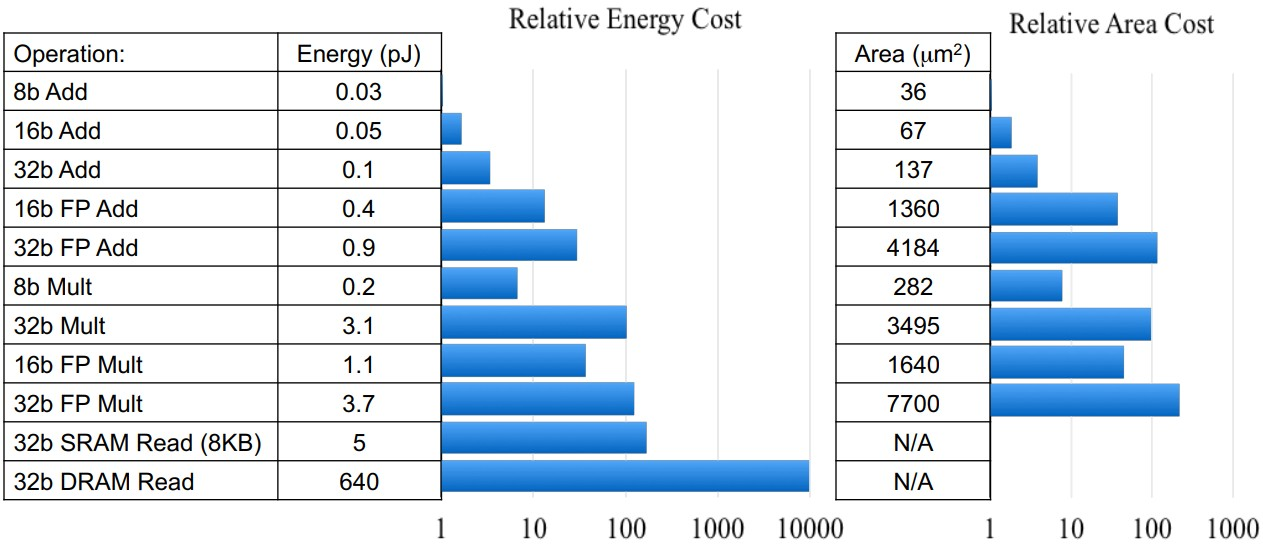
\includegraphics[width=\textwidth]{figures/chapter_4/quantization.jpg}
% \caption{Energy consumption \citep{dally2015high}}
% \label{fig.quantization}
% \end{figure}

% Pruning is a common methodology that induces sparsity in weights and activations. Weights that match the pruning criteria are assigned a value of zero. Prior research demonstrates that both fully connected layer and
% convolutional layer can be pruned, reducing the number of connections by 9× to 13× without loss of accuracy \citep{han2015learning}. After pruning, we have a simplified neural network for efficient inference.

% \begin{figure}[H]
% \centering
% 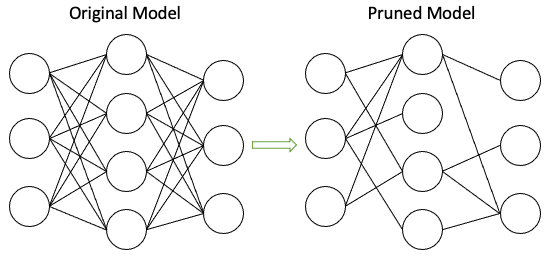
\includegraphics[scale=0.5]{figures/chapter_4/pruning.png}
% \caption{Pruning Neural Networks}
% \label{fig.pruning}
% \end{figure}

% Knowledge distillation is a model compression method in which a small model is trained to mimic a pre-trained, larger model. Sometimes this is referred to as "teacher-student", where the large model is the teacher and the small model is the student. Knowledge is transferred from the teacher model to the student by minimizing a loss function in which the target is the distribution of class probabilities predicted by the teacher model.

% In chapter 5, we'll try to deploy object detection and tracking system on hardware using both hardware accelerator and model compression.

% \clearpage

% \section{Adversarial Robustness}
% \label{sec:robusness}

% Deep learning models are robust if there is no obvious accuracy drop under adversarial attacks. Intuitively, quantization that uses 8-bit integers to represent weights and activations should improve model robustness, because unperceivable small perturbations can be neutralized after quantization. For instance, the original input 1.0 plus a small perturbation 0.01 is still 1.0 after quantization. However, prior research unveils that deep learning models are more vulnerable after quantization, which is counterintuitive.

% \begin{figure}[H]
% \centering
% 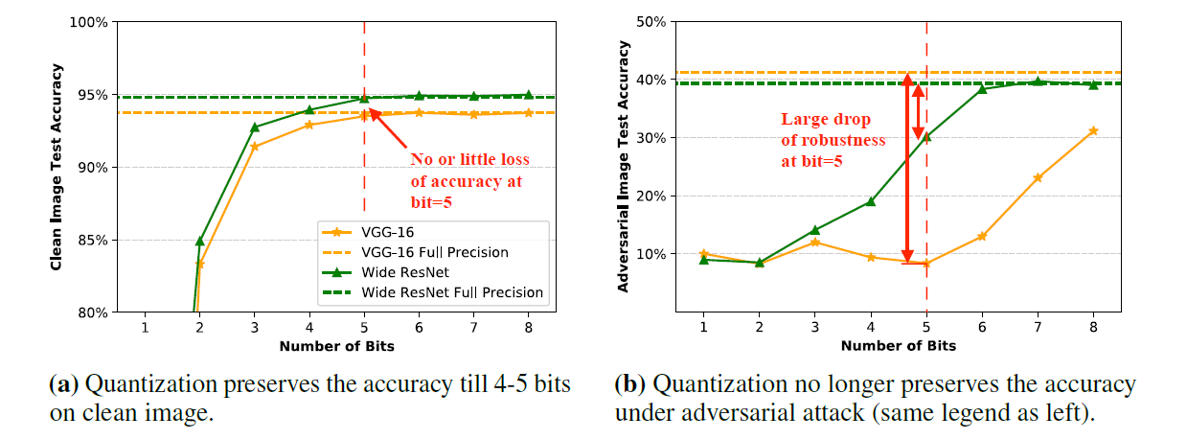
\includegraphics[width=\textwidth]{figures/chapter_4/robust_quantization.png}
% \caption{Deep Neural Networks become more vulnerable after quantization}
% \label{fig.qunatization_robustness}
% \end{figure}

% To improve model robustness, prior research suggests that the error is caused by the error amplification effect, and the robustness can be preserved by adding a Lipschitz regularization.

% \begin{figure}[H]
% \centering
% 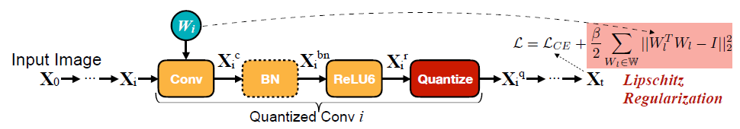
\includegraphics[width=\textwidth]{figures/chapter_4/defensive_quantization.png}
% \caption{Defensive Quantization \citep{lin2019defensive}}
% \label{fig.defensive_quantization}
% \end{figure}

% However, other research proposes that it is the batch normalization layer that makes the model more robust \citep{chai2021separating}. Thus, this is still an active research area that requires further investigation.

% In chapter 5, we'll further investigate the effect of quantization, pruning, and distillation on the effect of robustness in the application of adversarial tracking.

\clearpage

% \printbibliography[
%   keyword={chapter_tracking}, heading=subbibintoc, resetnumbers=true
% ]